\subsection{1T-APS}

The authors of \cite{FDSOI1} propose an active pixel sensor (APS) comprised of a single transistor. The device is fabricated using 22-nm FD-SOI technology and it is tested with light of wavelength of $520\unit{\nano\meter}$ \cite{FDSOI1}. The proposed sensor belongs to a class of devices referred to as \textsl{charge-coupled devices} (CCD) \cite{FDSOI1}.\par
CCD-based sensors take advantage of electrical charge accumulated during measurements \cite{CCD}. Later, the charge is transformed into voltage or current, amplified and measured \cite{CCD}. The proposed device is shown in figure \ref{fig:FDSOI:TEM}.\par
Traditional CMOS pixel sensors consist of a photodiode with four auxiliary transistors \cite{FDSOI1}\cite{1715616}. The proposed pixel integrates the photodiode, the reset function, and the signal amplification in a single device. Beneath the box there is an n-well on a p-substrate. This pn junction acts as the photodiode \cite{FDSOI1}.\par

\begin{figure}[h!]
	\centering
	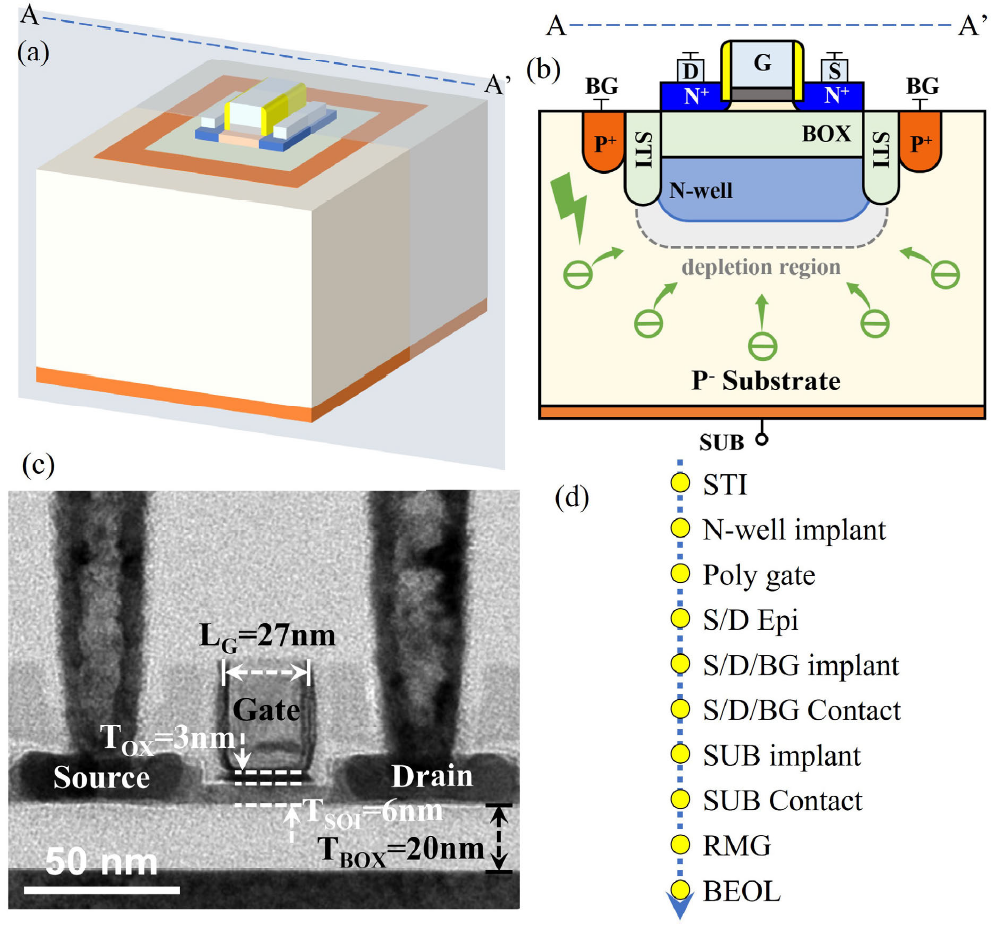
\includegraphics[width=0.9\linewidth]{assets/FD-SOI/1T_Pixel_Sensor/TEM.png}
	\caption{ (a) Schematic 3D structure and (b) 2D cross-section of 1T-APS. (c) XTEM image and (d) the simplified process flow. Taken from \cite{FDSOI1}.}
	\label{fig:FDSOI:TEM}
\end{figure}

\subsubsection{Operation}

	A negative voltage pulse is applied to the substrate (SUB) and back-gaet (BG) electrodes. This pulse leads to the formation of a depletion region on the pn junction as shown in figure \ref{fig:FDSOI:TEM} \cite{FDSOI1}. In the experiments performed by the authors, light of wavelength $\lambda=520\unit{\nano\meter}$ (green visible light) was used. When light hits the photodiode charges start to accumulate causing a variation of drain current, $I_d$, \cite{FDSOI1}. $I_d$ can be amplified, if needed, and measured to obtain the response of the sensor.\par
	The authors verified experimentally the successful reset of the sensor by zeroing the voltage at the SUB and BG electrodes and reapplying negative pulses to the same terminals \cite{FDSOI1}.\par
	It is demonstrated that the potential of the substrate is mainly controlled by the back-gate (BG) terminal \cite{FDSOI1}. Additionally, $V_{bg}$ controls the size of the depletion area \cite{FDSOI1}; thus, affecting the full-well capacity (FWC). Full-well capacity is a means of quantifying the total charge that can be stored in the photodiode well \cite{LEE2022108472}; i.e. beneath the BOX in this case. Hence, $V_{bg}$ and $V_{sub}$ can be used as tuning knobs for the sensor sensitivity \cite{FDSOI1}.\par

	\begin{figure}[h]
		\centering
		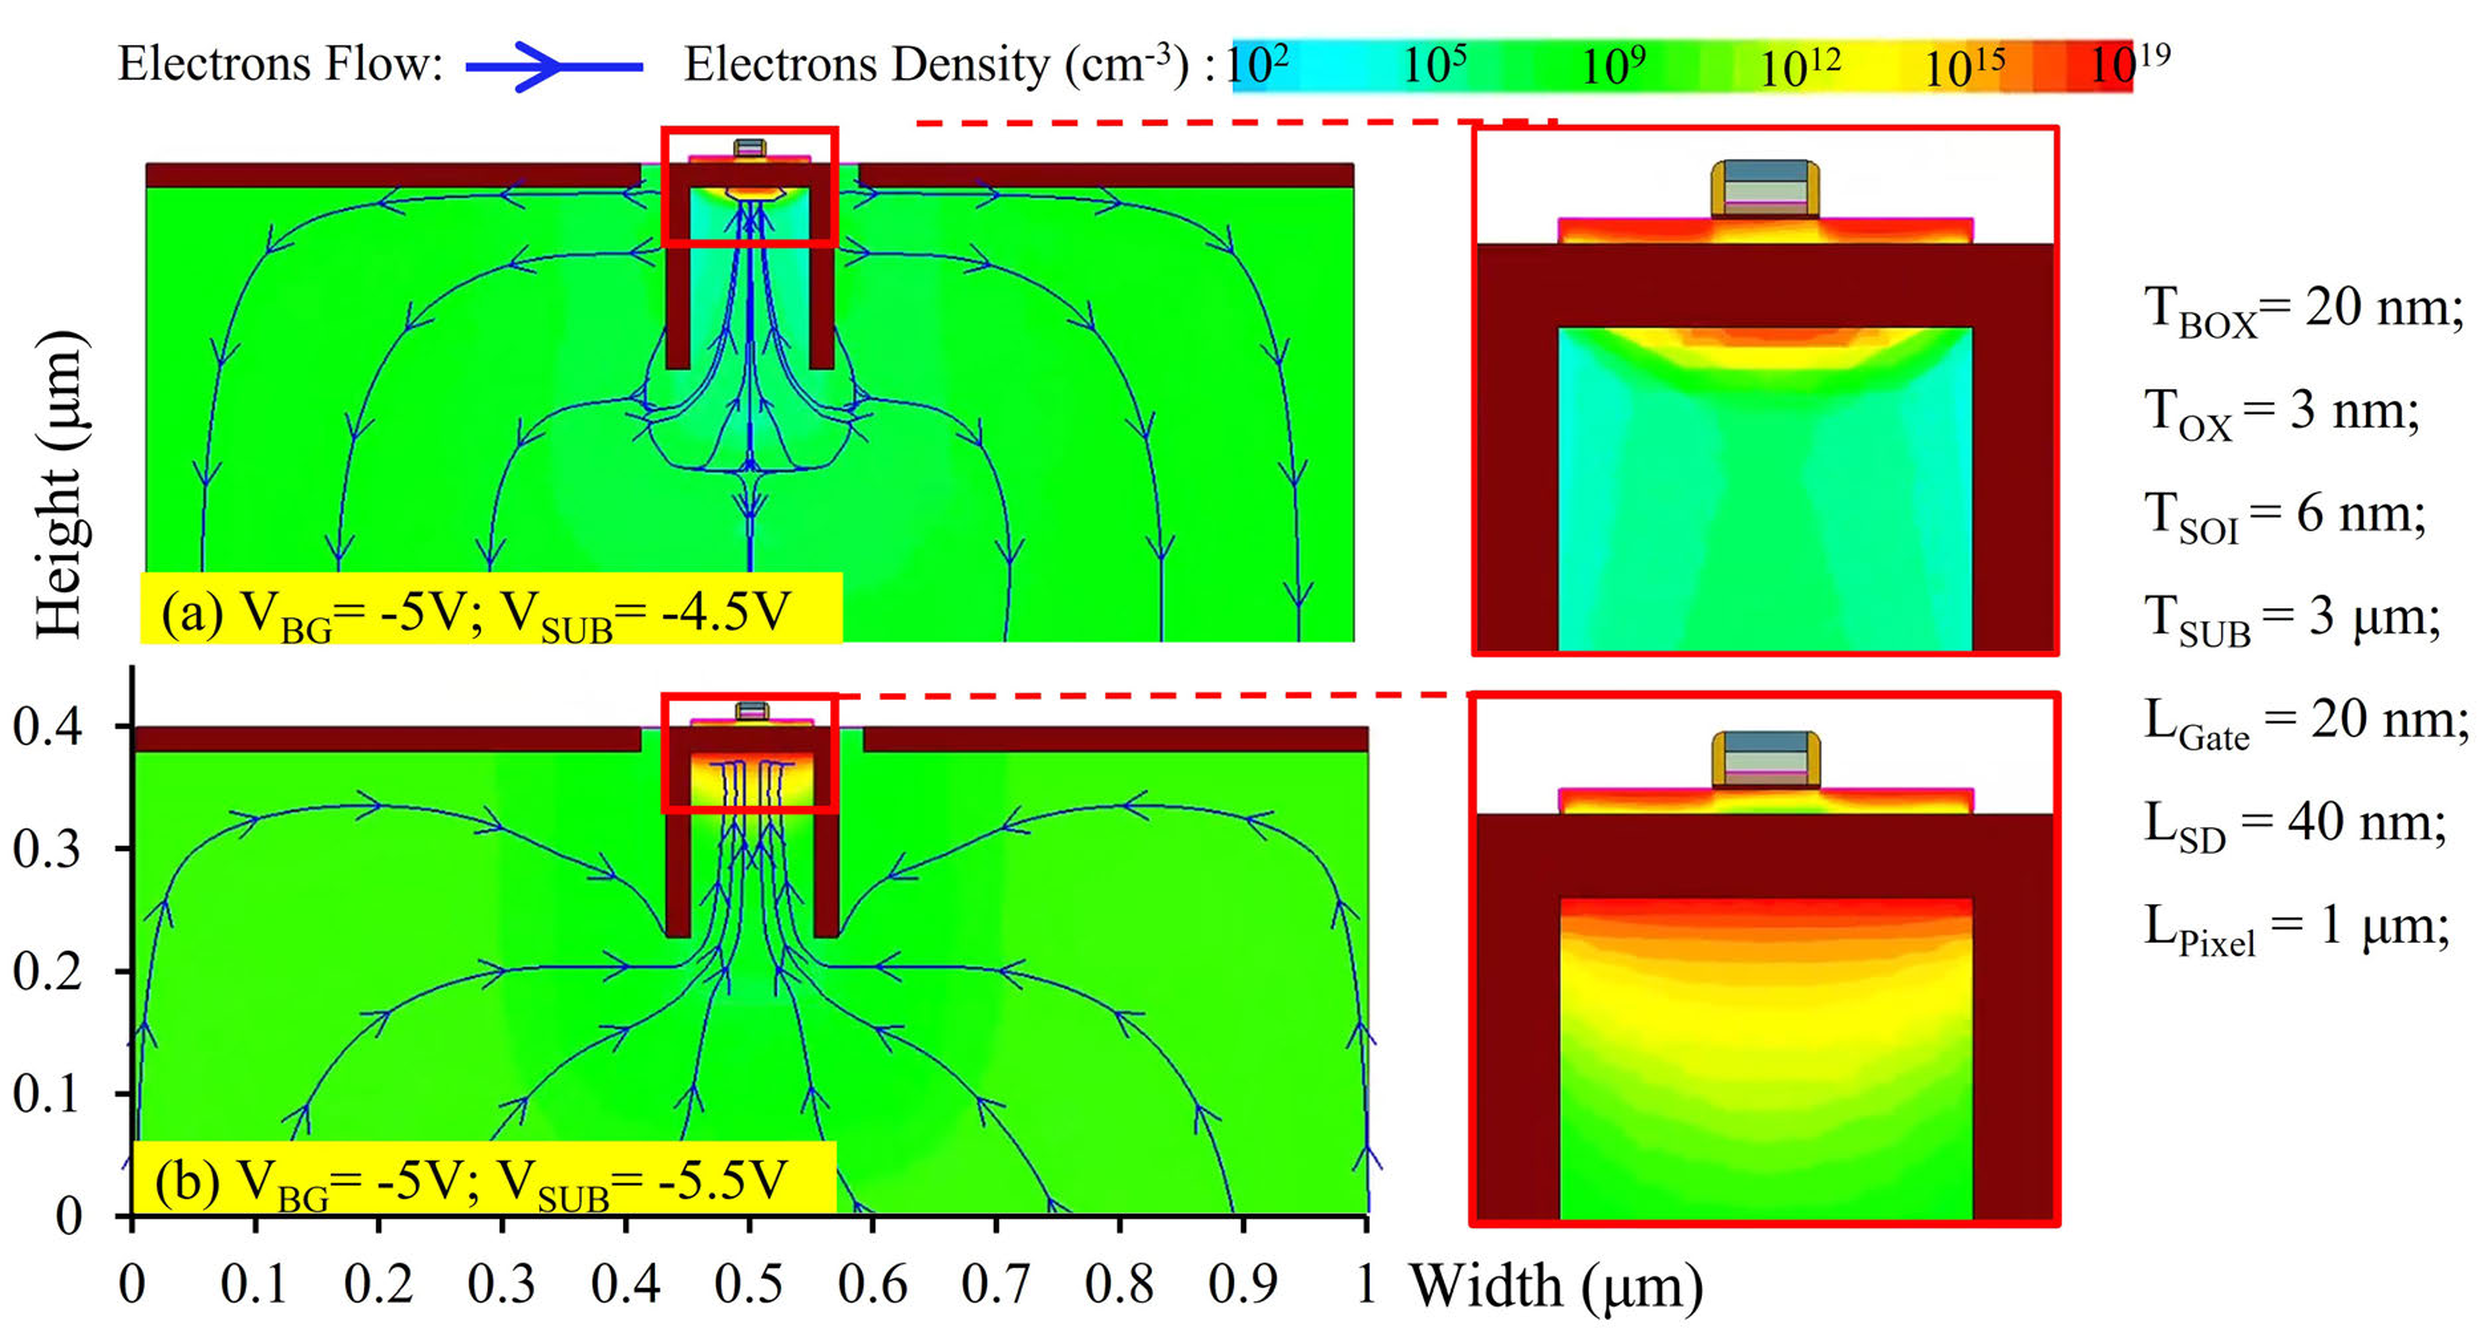
\includegraphics[width=0.9\linewidth]{assets/FD-SOI/1T_Pixel_Sensor/electrostatics.png}
		\caption{On the left: electron flow during exposure. On the right: electron distribution during exposure. Taken from \cite{FDSOI1}.}
		\label{fig:fdsoi:pixel:electrostatics}
	\end{figure}

	Figure \ref{fig:fdsoi:pixel:electrostatics} shows how the potential difference $V_{bg}-V_{sub}$ affects the flow of electrons from the substrate toward or away from the area beneath the BOX; hence, there is difference in the sensor's sensitivity \cite{FDSOI1}. $V_{bg}\lneqq V_{sub}$ forces the substrate-electrons away from the well beneath the BOX \cite{FDSOI1}. On the other hand, $V_{bg}\gneqq V_{sub}$ pushes electrons toward the well increasing the accumulated charge and increasing sensitivity \cite{FDSOI1}.\par